\documentclass[12pt]{article}
\usepackage{graphicx}
\usepackage{amssymb}
\usepackage{epstopdf}
\usepackage{amsmath}
\usepackage{multicol}
\usepackage{tcolorbox}
\usepackage{geometry}
\usepackage{enumitem}
\usepackage{fancyhdr}

\DeclareGraphicsRule{.tif}{png}{.png}{`convert #1 `dirname #1`/`basename #1 .tif`.png}

\textwidth = 6.5 in
\textheight = 9 in
\oddsidemargin = 0.0 in
\evensidemargin = 0.0 in
\topmargin = -23pt
\headheight = 0.0 in
\headsep = 0.0 in
\parskip = 0.2in
\parindent = 0.0in
\pagestyle{fancy}
\pagenumbering{gobble}

\newtheorem{theorem}{Theorem}
\newtheorem{corollary}[theorem]{Corollary}
\newtheorem{definition}{Definition}
%\includegraphics [height=50mm, width=50mm]{PathInt.jpg}
\title{Title} 

\begin{document}


 Name:
 \begin{center}\large{5.4 Theorems about Definite Integrals}\end{center}



\begin{enumerate}
\item The function $f(x)$ is graphed below. Note that it is made of two half circles.\\
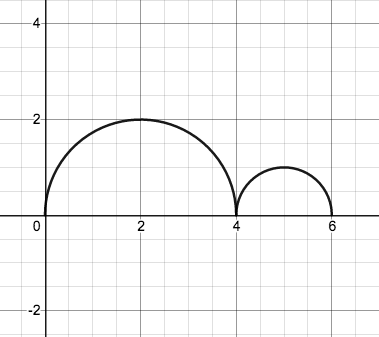
\includegraphics [scale=.4]{5_4_circ}
	\begin{enumerate}
	\item Find $\displaystyle \int_{0}^{6}f\left(x\right)dx$. 
	\item How does this illustrate the property $\displaystyle \int_{a}^{b}f\left(x\right)dx+\int_{b}^{c}f\left(x\right)dx=\int_{a}^{c}f\left(x\right)dx$?
	\end{enumerate}
\vfill
\item Which of the following integrals are positive? Why?\\

\noindent\begin{minipage}{0.3\textwidth}% adapt widths of minipages to your needs
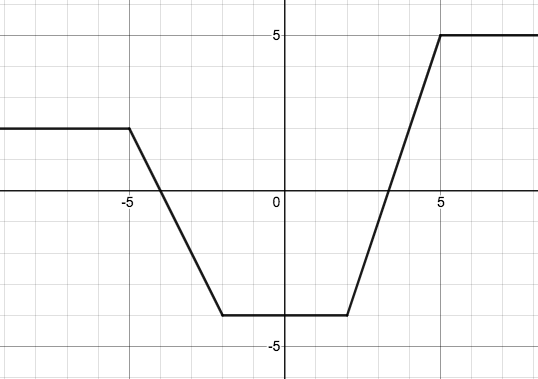
\includegraphics [scale=.4]{5_4_piece}
\end{minipage}%
\hspace{40mm}
\begin{minipage}{0.6\textwidth}
(a) $\displaystyle \int_{2}^{0}f\left(x\right)dx$\\\

(b) $\displaystyle \int_{5}^{10}f\left(x\right)dx$\\

(c) $\displaystyle \int_{-10}^{-5}f\left(x\right)dx$\\

(d) $\displaystyle \int_{-5}^{-10}f\left(x\right)dx$\\

\end{minipage}
\vfill
\newpage
~
\item Given that $\displaystyle \int_{0}^{1.25}\cos\left(x^{2}\right)dx=0.98$ and $\displaystyle \int_{0}^{1}\cos\left(x^{2}\right)dx=0.90$. Find the following values.\\
\noindent\begin{minipage}{0.3\textwidth}% adapt widths of minipages to your needs
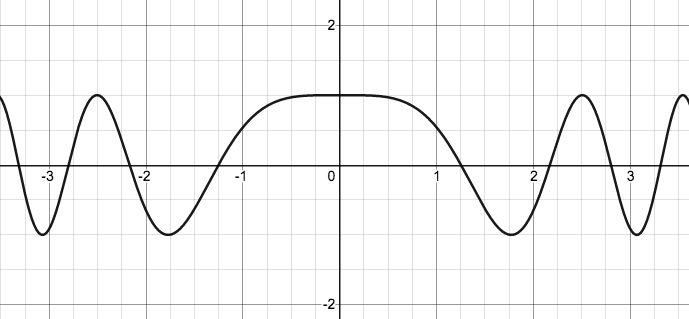
\includegraphics [scale=.4]{5_4_cos}
\end{minipage}%
\hspace{60mm}
\begin{minipage}{0.6\textwidth}
(a) $\displaystyle \int_{1}^{1.25}\cos\left(x^{2}\right)dx$\\\

(b) $\displaystyle \int_{-1}^{1}\cos\left(x^{2}\right)dx$\\

(c) $\displaystyle \int_{1.25}^{-1}\cos\left(x^{2}\right)dx$\\

\end{minipage}
\vfill

\item The functions $\displaystyle f\left(x\right)=x^{2}$ and $\displaystyle g\left(x\right)=x+3$ are graphed below. \\
	
	\noindent\begin{minipage}{0.3\textwidth}% adapt widths of minipages to your needs
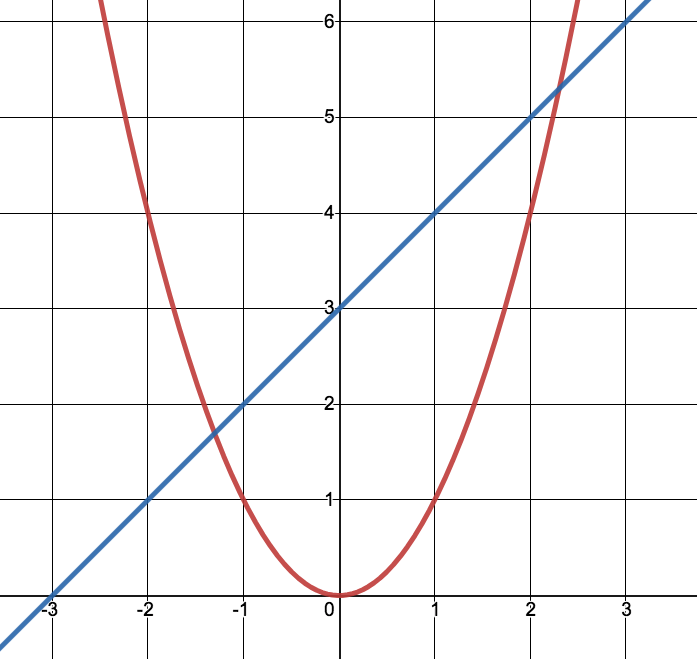
\includegraphics [scale=.24]{5_4_area}
\end{minipage}%
\hspace{10mm}
\begin{minipage}{0.6\textwidth}
(a)  Write and integral that represents the area between $\displaystyle f\left(x\right)=x^{2}$ and $\displaystyle g\left(x\right)=x+3$.\\
\vspace{10mm}\\
(b) Use FTC to compute the integral.\\

\end{minipage}
]
	\vfill
\item Find the average value of $f(x)$ on the interval $0\le x\le4$ when you know that $\displaystyle \int_{0}^{4}f\left(x\right)dx=9.22667$.\\
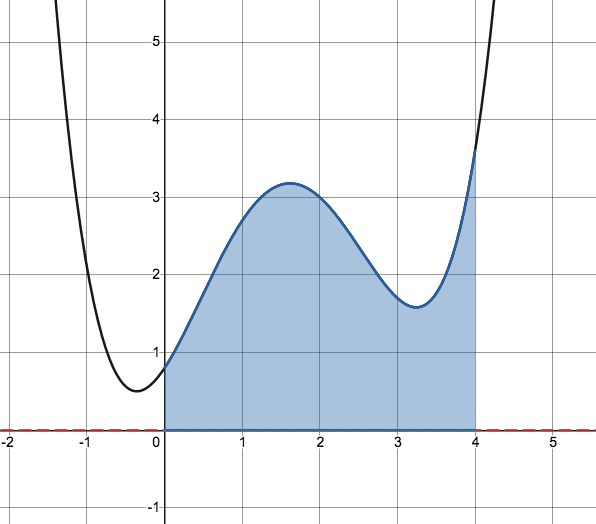
\includegraphics [scale=.24]{5_4_average}
	
\end{enumerate}
\end{document} 
%%%%%%%%%
\item Use diagrams and/or theorems to justify each of the following properties. 

	\begin{enumerate}
	\item $\displaystyle \int_a^c f(x)\,dx +\int_c^bf(x)\,dx =\underline{\hspace{4cm}} $\\
	\vfill
	\item $\displaystyle \int_a^a f(x)\,dx=\underline{\hspace{4cm}} $\\
	\vfill
	\item $\displaystyle \int_b^a f(x)\,dx=- \int_a^b f(x)\,dx$\\
	\vfill
	\item $\displaystyle \int_a^b kf(x)\,dx=k\int_a^b f(x)\,dx$\\
	(where $k$ is a constant)
	\vfill	
	\item $\displaystyle \int_a^b f(x)+g(x)\,dx=\int_a^b f(x)\,dx+ \int_a^b g(x)\,dx $\\
	\vfill	
	\item $\displaystyle \int_a^b f(x)-g(x)\,dx=\int_a^b f(x)\,dx-\int_a^b g(x)\,dx$\\
	\vfill	
	%\item If $f(x)<g(x)$ for all $a\leq x \leq b$, then $\displaystyle \int_a^b f(x)\,dx \leq   \int_a^b g(x)\,dx$.\\
	%\vfill	
	%\item If $m\leq f(x) \leq M$ for all $a\leq x \leq b$, then $\displaystyle \underline{\hspace{2cm}} \leq \int_a^b f(x)\,dx \leq \underline{\hspace{2cm}}.  $\\
	%\vfill	
	\item The average value of $f$ from $a$ to $b$ is $\displaystyle \frac{1}{b-a} \int_a^b f(x)\,dx$.
	\vfill
	\end{enumerate}
\newpage




\item Assume that $\displaystyle \int_a^b f(x)\,dx=9$, $\displaystyle \int_b^c f(x)\,dx=-7$, $\displaystyle \int_a^b (f(x))^2\,dx=36$, and\\ $\displaystyle \int_a^b g(x)\,dx=-2$. Use this information to calculate each of the following, or explain why there is not enough information to do so.
	\begin{enumerate}
	\item $\displaystyle \int_a^c f(x)\,dx$\\
	
	\item $\displaystyle \int_{-a}^{-b} f(x)\,dx$\\
	
	\item $\displaystyle \int_b^c |f(x)|\,dx$\\
	
	\item $\displaystyle \int_a^b (f(x))^2\,dx-  \left(\int_a^b f(x)\,dx \right)^2$\\
	
	\item $\displaystyle \int_a^b (2f(x)-g(x))\,dx$\\
		
	\end{enumerate}

\item In the year 2018, the population of Oregon was modeled by the function\\ $P=f(t)=4.191(1.014)^t$, where $P$ is in millions of people and $t$ is in years since 2014. Use this function to predict the average population of Oregon between the years 2015 and 2020.
\vfill

\item Using your calculator or desmos, find the area enclosed by the curves $y=2\cos(x)$ and $y=x^2+x$.
\vfill


\begin{tcolorbox}
\textbf{Warm-up: } Solve the following equations for $t$.
\begin{multicols}{2}
\begin{enumerate}
\item $(t+1)^2=9$
\item $tx+x^2=5$
\end{enumerate}
\end{multicols}
\end{tcolorbox}

MINIPAGE
\noindent\begin{minipage}{0.3\textwidth}% adapt widths of minipages to your needs
try 1
\end{minipage}%
\hspace{40mm}
\begin{minipage}{0.6\textwidth}
a) $f'(2)=$\\\

b) $f'(4)=$\\

c) $f'(6)=$\\

d) $f'(7)=$\\

e) $f'(8)=$
\end{minipage}
